\section{Tareas Posteriores de SBERT}
\label{sec:sbert}

El embedding de oraciones se construye sobre entrenamiento estilo Siamese \citep{reimers_sentence-bert_2019}. Para el par de oraciones $(s_1,s_2)$ con embeddings $(e_1,e_2)$:
\[
\text{cos}(e_1,e_2)=\frac{e_1^\top e_2}{\|e_1\|\|e_2\|}
\]
y pérdida coseno estilo regresión:
\[
\mathcal{L}_{\text{cos}}=\left(\text{cos}(e_1,e_2)-y\right)^2
\]
con $y\in[-1,1]$ en este pipeline.

Modos posteriores soportados:
\begin{itemize}[leftmargin=*]
    \item \textbf{Similitud}: puntuación por pares entre dos oraciones.
    \item \textbf{Búsqueda}: $k$ vecinos más cercanos sobre un corpus.
    \item \textbf{Clustering}: agrupación de embeddings (ej., k-means).
    \item \textbf{Codificación}: exportación persistente de embeddings para recuperación posterior.
\end{itemize}

\begin{figure}[t]
\centering
\fitfigure{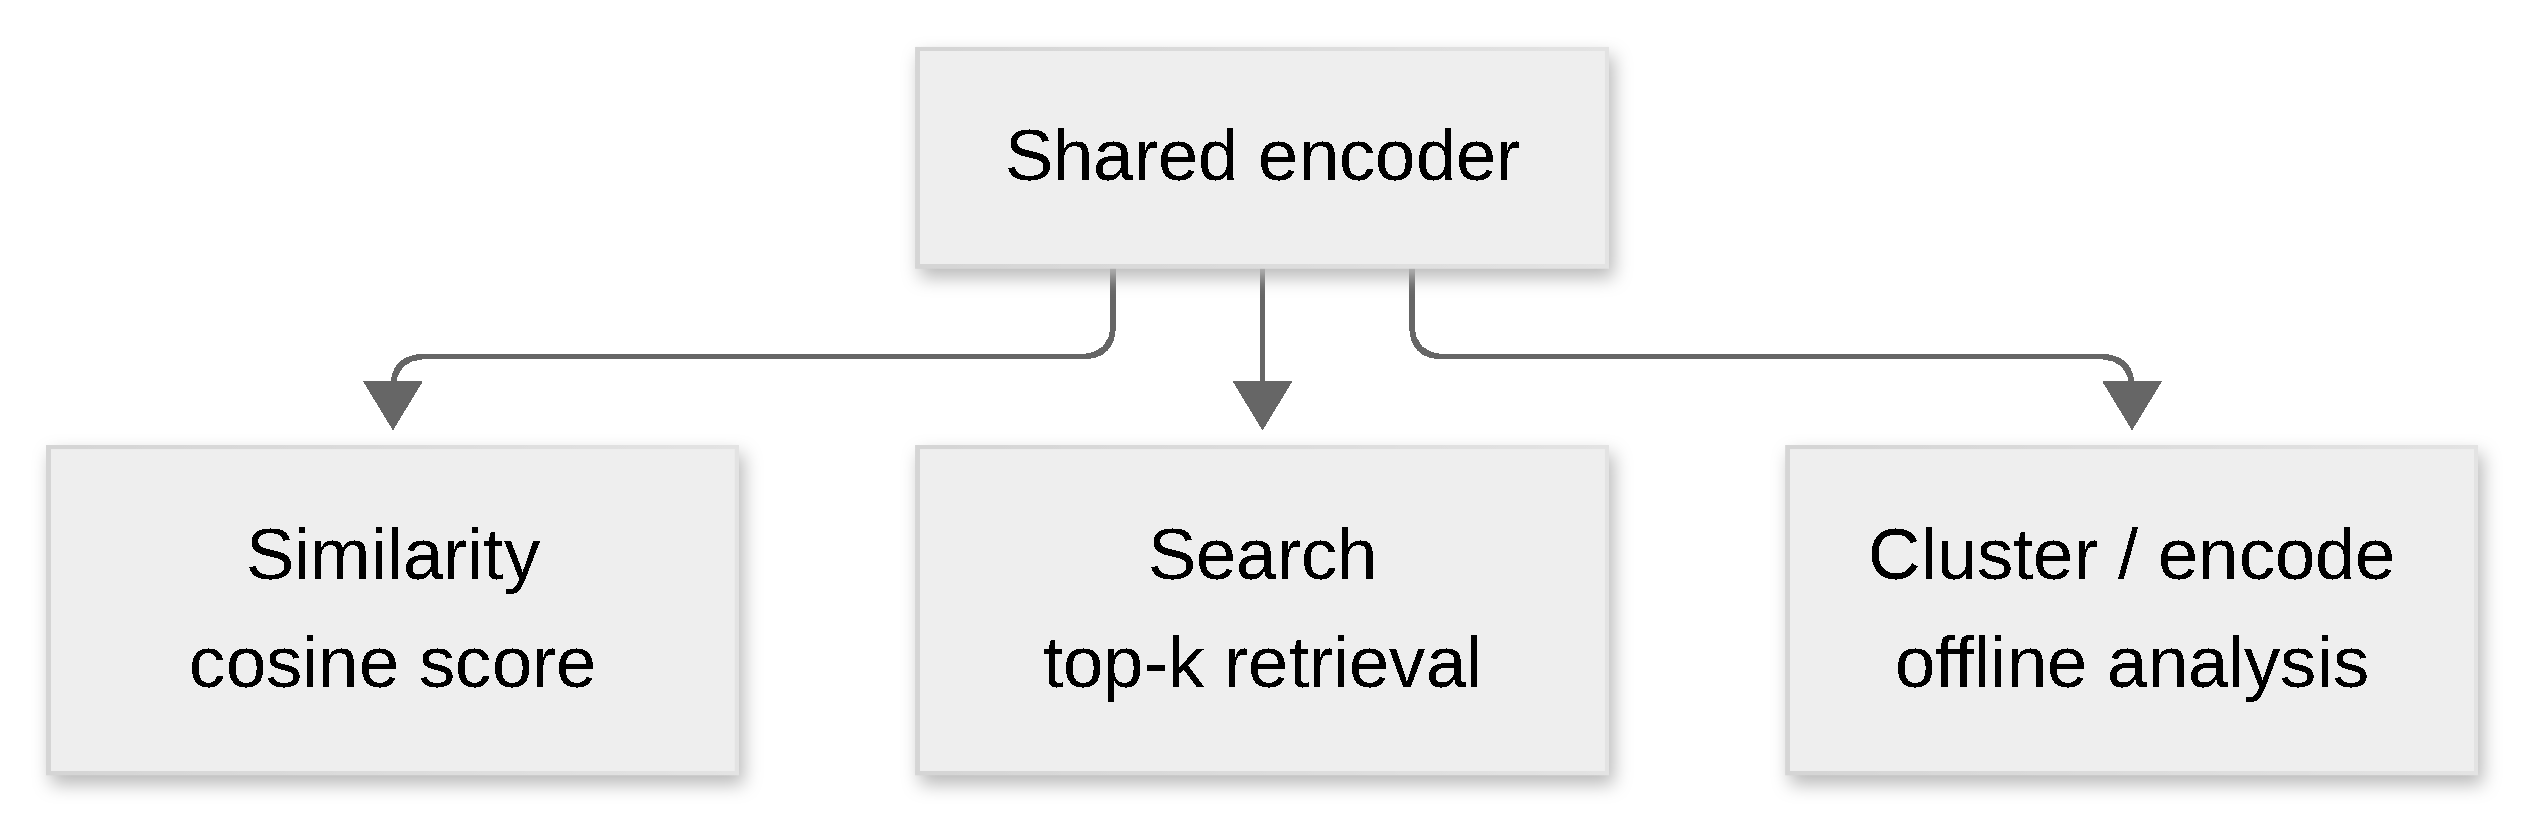
\includegraphics{../paper/figures/sbert-modes.pdf}}
\caption{Reutilización del flujo de trabajo SBERT. Un único codificador soporta puntuación de pares en línea, recuperación sobre corpus, clustering y exportación persistente de embeddings.}
\label{fig:sbert-modes}
\end{figure}

El pseudocódigo del enrutador de modo de inferencia SBERT---despachando entre los modos de similitud, búsqueda, cluster y codificación sobre un codificador compartido---se remite al Apéndice~\ref{sec:annex-norm-bitnet-mod}.

